\documentclass[10pt,journal,compsoc]{IEEEtran}
\usepackage[utf8]{inputenc}

% *** CITATION PACKAGES ***
%
\ifCLASSOPTIONcompsoc
  % The IEEE Computer Society needs nocompress option
  % requires cite.sty v4.0 or later (November 2003)
  \usepackage[nocompress]{cite}
\else
  % normal IEEE
  \usepackage{cite}
\fi
\usepackage{graphicx}
\usepackage{caption}
\usepackage{eurosym} 
\renewcommand{\tablename}{Tab.}
\graphicspath{ {images/} }
% *** GRAPHICS RELATED PACKAGES ***
%
\ifCLASSINFOpdf
  
\else
 
\fi
\newcommand\MYhyperrefoptions{bookmarks=true,bookmarksnumbered=true,
pdfpagemode={UseOutlines},plainpages=false,pdfpagelabels=true,
colorlinks=true,linkcolor={black},citecolor={black},urlcolor={black},
pdftitle={Bare Demo of IEEEtran.cls for Computer Society Journals},%<!CHANGE!
pdfsubject={Typesetting},%<!CHANGE!
pdfauthor={Michael D. Shell},%<!CHANGE!
pdfkeywords={Computer Society, IEEEtran, journal, LaTeX, paper,
             template}}%<^!CHANGE!

\hyphenation{op-tical net-works semi-conduc-tor}


\begin{document}

\title{Sistema domótico IoT basado en Raspberry Pi y control remoto por Telegram}
\author{Jesús Gómez Bellido}

% for Computer Society papers, we must declare the abstract and index terms
% PRIOR to the title within the \IEEEtitleabstractindextext IEEEtran
% command as these need to go into the title area created by \maketitle.
% As a general rule, do not put math, special symbols or citations
% in the abstract or keywords.
\IEEEtitleabstractindextext{%
\begin{abstract}
The abstract goes here.
\end{abstract}

% Note that keywords are not normally used for peerreview papers.
\begin{IEEEkeywords}
Computer Society, IEEE, IEEEtran, journal, \LaTeX, paper, template.
\end{IEEEkeywords}}


\maketitle


% To allow for easy dual compilation without having to reenter the
% abstract/keywords data, the \IEEEtitleabstractindextext text will
% not be used in maketitle, but will appear (i.e., to be "transported")
% here as \IEEEdisplaynontitleabstractindextext when compsoc mode
% is not selected <OR> if conference mode is selected - because compsoc
% conference papers position the abstract like regular (non-compsoc)
% papers do!
\IEEEdisplaynontitleabstractindextext
% \IEEEdisplaynontitleabstractindextext has no effect when using
% compsoc under a non-conference mode.


% For peer review papers, you can put extra information on the cover
% page as needed:
% \ifCLASSOPTIONpeerreview
% \begin{center} \bfseries EDICS Category: 3-BBND \end{center}
% \fi
%
% For peerreview papers, this IEEEtran command inserts a page break and
% creates the second title. It will be ignored for other modes.
\IEEEpeerreviewmaketitle


\ifCLASSOPTIONcompsoc
\IEEEraisesectionheading{\section{Introduction}\label{sec:introduction}}
\else
\section{Introduccion y objetivos}
\label{sec:introduction}
\fi

\IEEEPARstart En este Trabajo fin de Máster (TFM) vamos a tratar de ver el impacto que pueden generar las nuevas tecnologías que se están empezando a expandir.
Estas nuevas tecnologías tienen siempre en mente una perspectiva, el llamado "Internet of Things" (IoT) o Internet de las Cosas. 
Este es un término se refiere a la interconexión de dispositivos físicos, vehículos, edificios y otros objectos --embebidos con electrónica, software, sensores, actuadores y conexión a internet que permiten la recolección de datos.
Todo esto nos permite que los ordenadores interactúen con elementos de la vida real y ganen independencia de los seres humanos.

Bien es cierto, que el IoT va a suponer un gran impacto en cuanto a la industria y la investigación, pero no será menos para los ambientes domésticos ya que nos permite automatizar muchas funciones de nuestros hogares.
En este entorno tiene gran parte de importancia el uso de los \textit{smartphones}, pues son en muchos casos los encargados de comunicar a los seres humanos con nuestros dispositivos.

Otro de los dispositivos en auge y que han fomentado la automatización en los hogares son los micro-ordenadores, como son las Raspberry Pi, estos son dispositivos tremendamente versátiles y cada vez más potentes.


\subsection{Objetivos}
En el actual TFM, vamos buscar unos objetivos basándonos en IoT en un entorno doméstico.
Se realizará un sistema domótico básandonos en los principios del IoT.

Para llevar a cabo el primer objetivo, se va a usar una Raspberry Pi programandose en JavaScript
y viendo las posibilidades que este lenguaje nos proporciona en relación a Python, el cuál se puede decir que es el lenguaje de programación estándar para la Raspberry Pi.

El sistema domótico, realizará el control sobre persianas/toldos, basándose en las previsiones de servicios meteorológicos, prevaleciendo las acciones del usuario. El usuario también tendrá control sobre puertas, luces, el sistema de climatización y la alarma.

Por otro lado también se tendrá un control de presencia dentro de la casa, registrando las entradas y salidas de los usuarios mediante la MAC de su smartphone y el protocolo ARP. 

Por último, el control de nuestro sistema domótico se realizará mediante Telegram, las aplicaciones de mensajerías son algo indispensable hoy en día para las personas, así que viendo la API que este servicio de mensajería nos proporciona para realizar bots, parece interesante estudiar qué clase de posibilidades se nos abren con estos tres elementos.

\section{Arquitectura del sistema}
\begin{figure}[h]
\centering
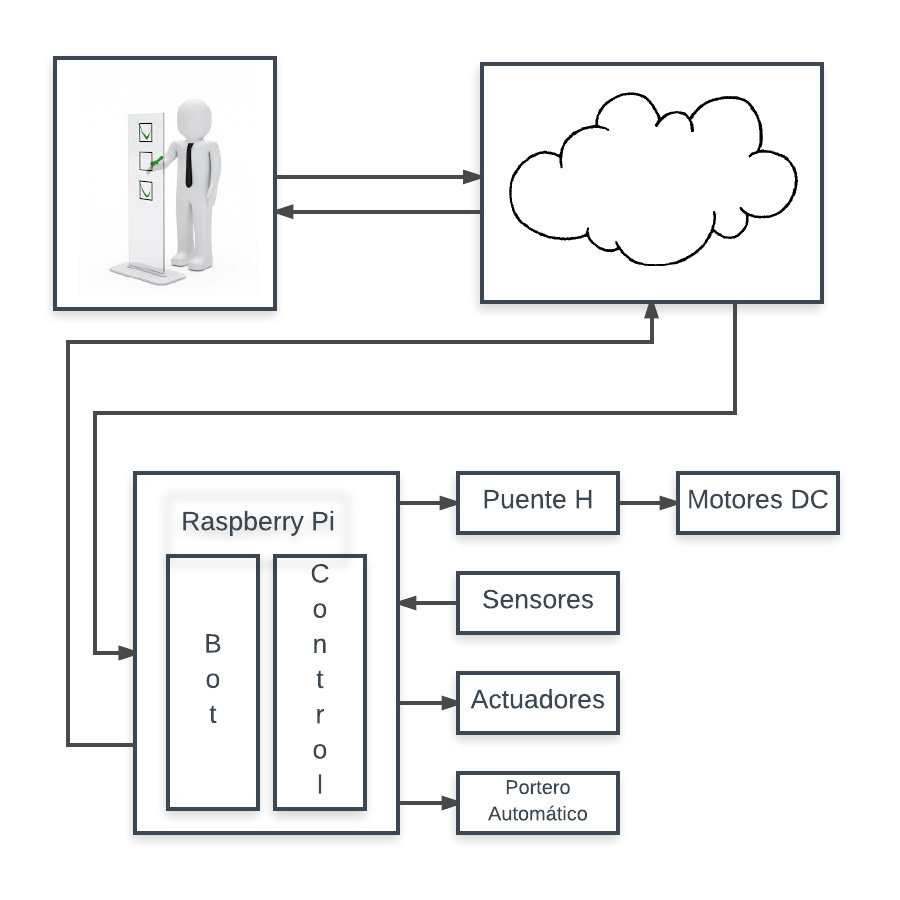
\includegraphics[scale=0.5]{ArqSist}
\caption{Arquitectura del sistema}
\label{fig:arqSist}
\end{figure}

En la figura \ref{fig:arqSist} se muestra la arquitectura del sistema que se va a desarrollar. Como vemos, el usuario no tiene contacto directo con el sistema. Pues aunque se encuentre la Raspberry Pi y el usuario en la misma red, la comunicación se estable con el servidor de telegram de por medio.

Una vez que el usuario envía un comando y el bot lo recibe, éste provoca un evento y envía la orden hacia la lógica de control. La cual actuará en consecuencia de su alrededor.

De igual forma que nosotros enviamos comandos al sistema, el sistema nos devolverá los diferentes datos que recoge por los sensores y servicios que se estén manejando en ese momento.


\section{Desarrollo Software}
The conclusion goes here.

\section{Pruebas de Rendimiento}
The conclusion goes here.

\section{Costes}
El tiempo desarrollo de este sistema domótico ha sido de 100 horas, tomando un precio por hora de 30\euro, tenemos un coste de desarrollo de 3000\euro.
Luego cada sistema tendría un coste fijo de:

\begin{table}[h]
\centering
\begin{tabular}{ccc}
Raspberry Pi & ........ & 50\euro \\
Sensores & ........ & 10\euro \\
Actuadores & ........ & 15\euro \\
Motores & ........ & 25\euro \\
\hline \\
Total & ........ & 100\euro \\
\end{tabular} 
\caption{Costes fijos}
\label{tab:CostesFij}
\end{table}

Para cubrir los costes que vemos en la tabla \ref{tab:CostesFij}, con la venta de 100 terminales, cada terminal debería tener un precio de 157,30\euro (IVA Incl.)

\section{Conclusion}
The conclusion goes here.

\hfill mds
 
\hfill August 26, 2015

\begin{thebibliography}{1}

\bibitem{IEEEhowto:kopka}
H.~Kopka and P.~W. Daly, \emph{A Guide to {\LaTeX}}, 3rd~ed.\hskip 1em plus
  0.5em minus 0.4em\relax Harlow, England: Addison-Wesley, 1999.

\end{thebibliography}
\end{document}


